\documentclass[11pt]{article} 
\usepackage[english]{babel}
\usepackage[utf8]{inputenc}
\usepackage[margin=0.5in]{geometry}
\usepackage{amsmath}
\usepackage{amsthm}
\usepackage{amsfonts}
\usepackage{amssymb}
\usepackage[usenames,dvipsnames]{xcolor}
\usepackage{graphicx}
%\usepackage[siunitx]{circuitikz}
\usepackage{tikz}
\usepackage[colorinlistoftodos, color=orange!50]{todonotes}
\usepackage{hyperref}
\usepackage[numbers, square]{natbib}
\usepackage{fancybox}
\usepackage{epsfig}
\usepackage{soul}
\usepackage[framemethod=tikz]{mdframed}
\usetikzlibrary{positioning, automata, backgrounds}
\usepackage[shortlabels]{enumitem}
\usepackage[version=4]{mhchem}
\usepackage{multicol}
\usepackage{forest}
\usepackage{mathtools}
\usepackage{comment}
\usepackage{enumitem}
\usepackage[utf8]{inputenc}
\usepackage[linesnumbered,ruled,vlined]{algorithm2e}
\usepackage{listings}
\usepackage{color}
\usepackage[numbers]{natbib}
\usepackage{subfiles}
%\usepackage{tkz-berge}
\usepackage{listings}
\lstset{
  basicstyle=\ttfamily,
  mathescape
}

\newtheorem{prop}{Proposition}[section]
\newtheorem{thm}{Theorem}[section]
\newtheorem{lemma}{Lemma}[section]
\newtheorem{cor}{Corollary}[prop]

\theoremstyle{definition}
\newtheorem{definition}{Definition}

\theoremstyle{definition}
\newtheorem{required}{Problem}

\theoremstyle{definition}
\newtheorem{ex}{Example}


\newcommand{\interval}[4]{\draw (#2, #1) -- (#3, #1); % Usage: \interval{height}{start}{end}{label}
\draw (#2, #1-0.11) -- (#2, #1+0.11); % draw left whisker
\draw (#3, #1-0.11) -- (#3, #1+0.11); % draw right whisker
\node[] at (#2-0.25, #1) {#4};
}

\setlength{\marginparwidth}{3.4cm}
%#########################################################

%To use symbols for footnotes
\renewcommand*{\thefootnote}{\fnsymbol{footnote}}
%To change footnotes back to numbers uncomment the following line
%\renewcommand*{\thefootnote}{\arabic{footnote}}

% Enable this command to adjust line spacing for inline math equations.
% \everymath{\displaystyle}

% _______ _____ _______ _      ______ 
%|__   __|_   _|__   __| |    |  ____|
%   | |    | |    | |  | |    | |__   
%   | |    | |    | |  | |    |  __|  
%   | |   _| |_   | |  | |____| |____ 
%   |_|  |_____|  |_|  |______|______|
%%%%%%%%%%%%%%%%%%%%%%%%%%%%%%%%%%%%%%%

\title{
\normalfont \normalsize 
\textsc{CSCI 3104 Fall 2021 \\ 
Instructor: Profs. Grochow and Waggoner} \\
[10pt] 
\rule{\linewidth}{0.5pt} \\[6pt] 
\huge Problem Set 2 \\
\rule{\linewidth}{2pt}  \\[10pt]
}
%\author{Your Name}
\date{}

\begin{document}
\definecolor {processblue}{cmyk}{0.96,0,0,0}
\definecolor{processred}{rgb}{200, 0, 0}
\definecolor{processgreen}{rgb}{0, 255, 0}
\DeclareGraphicsExtensions{.png}
\DeclareGraphicsExtensions{.gif}
\DeclareGraphicsExtensions{.jpg}

\maketitle


%%%%%%%%%%%%%%%%%%%%%%%%%
%%%%%%%%%%%%%%%%%%%%%%%%%%
%%%%%%%%%%FILL IN YOUR NAME%%%%%%%
%%%%%%%%%%AND STUDENT ID%%%%%%%%
%%%%%%%%%%%%%%%%%%%%%%%%%%
\noindent
Due Date \dotfill \textbf{September 14, 2021} \\
Name \dotfill \textbf{Didi Trifonova} \\
Student ID \dotfill \textbf{109388776} \\
%Collaborators \dotfill \textbf{List Your Collaborators Here}

\tableofcontents

\section{Instructions}
 \begin{itemize}
	\item The solutions \textbf{must be typed}, using proper mathematical notation. We cannot accept hand-written solutions. \href{http://ece.uprm.edu/~caceros/latex/introduction.pdf}{Here's a short intro to \LaTeX.}
	\item You should submit your work through the \textbf{class Canvas page} only. Please submit one PDF file, compiled using this \LaTeX \ template.
	\item You may not need a full page for your solutions; pagebreaks are there to help Gradescope automatically find where each problem is. Even if you do not attempt every problem, please submit this document with no fewer pages than the blank template (or Gradescope has issues with it).

	\item You are welcome and encouraged to collaborate with your classmates, as well as consult outside resources. You must \textbf{cite your sources in this document.} \textbf{Copying from any source is an Honor Code violation. Furthermore, all submissions must be in your own words and reflect your understanding of the material.} If there is any confusion about this policy, it is your responsibility to clarify before the due date. 

	\item Posting to \textbf{any} service including, but not limited to Chegg, Reddit, StackExchange, etc., for help on an assignment is a violation of the Honor Code.

	\item You \textbf{must} virtually sign the Honor Code (see Section \ref{HonorCode}). Failure to do so will result in your assignment not being graded.
\end{itemize}


\section{Honor Code (Make Sure to Virtually Sign)} \label{HonorCode}

\begin{required}
\begin{itemize}
\item My submission is in my own words and reflects my understanding of the material.
\item Any collaborations and external sources have been clearly cited in this document.
\item I have not posted to external services including, but not limited to Chegg, Reddit, StackExchange, etc.
\item I have neither copied nor provided others solutions they can copy.
\end{itemize}

%\noindent In the specified region below, clearly indicate that you have upheld the Honor Code. Then type your name. 
\end{required}

\begin{proof}[Agreed (Didi Trifonova)]
\end{proof}



\newpage
\section{Standard 3- Dijkstra's Algorithm}

\subsection{Problem \ref{Dijkstra0}}
\begin{required} \label{Dijkstra0}
Consider the weighted graph $G(V, E, w)$ pictured below. Work through Dijkstra's algorithm on the following graph, using the source vertex $E$. 
\begin{itemize}
\item Clearly include the contents of the priority queue, as well as the distance from $E$ to each vertex at each iteration.
\item If you use a table to store the distances, clearly label the keys according to the vertex names rather than numeric indices (i.e., \texttt{dist[`B']} is more descriptive than \texttt{dist[`1']}).
\item You do \textbf{not} need to draw the graph at each iteration, though you are welcome to do so. [This may be helpful scratch work, which you do not need to include.]
\end{itemize}


\begin{center}
\begin {tikzpicture}[-latex, auto, node distance =2 cm and 3cm, semithick]
\tikzstyle{blue}=[circle ,top color =white , bottom color = processblue!20 ,draw,processblue , text=blue , minimum width =1 cm];
\tikzstyle{red}=[circle ,top color =white , bottom color = processred!20 ,draw, processred , text=blue , minimum width =1 cm];
\tikzstyle{green}=[circle ,top color =white , bottom color = processgreen!20 ,draw, processgreen , text=blue , minimum width =1 cm];

	\node[blue] (A) {$A$};
	\node[blue] (C) [below right = of A] {$C$};
	\node[blue] (B) [below right = of C] {$B$};
	\node[blue] (E) [below left = of A] {$E$};
	\node[blue] (D) [below left = of E] {$D$};
	\node[blue] (H) [below right = of D] {$H$};
	\node[blue] (F) [right = of H] {$F$};

	\path (A) edge node[above] {$3$} (C);
	\path (E) edge node[left] {$9$} (A);

	\path (C) edge node[above] {$3$} (B);
	\path (B) edge node[below] {$6$} (F);

	\path (E) edge node[above] {$15$} (C);
	\path (C) edge node[above] {$2$} (F);

	\path (H) edge node[above] {$4$} (D);

	\path (E) edge node[above] {$20$} (F);
	\path (E) edge node[right] {$9$} (H);
	\end{tikzpicture}  
\end{center}

\end{required}

\begin{proof}[Answer]
\begin{enumerate}
\begin{lstlisting}

1. Priority queue: E
    distance[E] = 0
    distance of all other vertices = $\infty$
    
2. Priority queue:  H,A,C,F 
    distance[E] = 0
    distance[H] = 9 
    distance[A] = 9 
    distance[C] = 15
    distance[F] = 20 
    distance of all other vertices = $\infty$

3. Priority queue: A,D,C,F
    distance[E] = 0
    distance[H] = 9 
    distance[A] = 9 
    distance[C] = 15
    distance[F] = 20 
    distance[D] = 13
    distance of all other vertices = $\infty$
    
4. Priority queue: C,D,F
    distance[E] = 0
    distance[H] = 9 
    distance[A] = 9 
    distance[C] = 12
    distance[F] = 20 
    distance[D] = 13
    distance of all other vertices = $\infty$
    
5. Priority queue: D,F,B
    distance[E] = 0
    distance[H] = 9 
    distance[A] = 9 
    distance[C] = 12
    distance[F] = 14
    distance[D] = 13
    distance[B] = 15
    
6. Priority queue: F,B
    distance[E] = 0
    distance[H] = 9 
    distance[A] = 9 
    distance[C] = 12
    distance[F] = 14
    distance[D] = 13
    distance[B] = 15

7. Priority queue: B
    distance[E] = 0
    distance[H] = 9 
    distance[A] = 9 
    distance[C] = 12
    distance[F] = 14
    distance[D] = 13
    distance[B] = 15
    
8. Priority queue: Empty
    distance[E] = 0
    distance[H] = 9 
    distance[A] = 9 
    distance[C] = 12
    distance[F] = 14
    distance[D] = 13
    distance[B] = 15
    

\end{lstlisting}

\end{enumerate}
\end{proof}





\newpage
\subsection{Problem \ref{Dijkstra2}} 
\begin{required} \label{Dijkstra2}
You have three batteries, with 4200, 2700, and 1600 mAh (milli-Amp-hours), respectively. The 2700 and 1600-mAh batteries are fully charged (containing 2700 mAh and 1600 mAh, respectively), while the 4200-mAh battery is empty, with 0 mAh. You have a battery transfer device which has a ``source'' battery position and a ``target'' battery position. When you place two batteries in the device, it instantaneously transfers as many mAh from the source battery to the target battery as possible. Thus, this device stops the transfer either when the source battery has no mAh remaining or when the destination battery is fully charged (whichever comes first).  \\

\noindent But battery transfers aren't free! The battery device is also hooked up to your phone by bluetooth, and automatically charges you a number of cents equal to however many mAh it just transfered.  \\
	
\noindent The goal in this problem is to determine whether there exists a sequence of transfers that leaves exactly 1200 mAh either in the 2700-mAh battery or the 1600-mAh battery, and if so, how little money you can spend to get this result. \\

\noindent Do the following.
\begin{enumerate}[label=(\alph*)]
\subsubsection{Problem 3\ref{Dijkstra2a}}
\item \label{Dijkstra2a} Rephrase this is as a graph problem. Give a precise definition of how to model this problem as a graph, and state the specific question about this graph that must be answered. [\textbf{Note:} While you are welcome to draw the graph, it is enough to provide 1-2 sentences clearly describing what the vertices are and when two vertices are adjacent. If the graph is weighted, clearly specify what the edge weights are.]

\begin{proof}[Answer] $ $
\begin{enumerate}
    \item Let the three batteries be referenced as A (which holds 1600 mAh), B (which holds 2700 mAh), and C (which holds 4200 mAh). 
    \item Let the vertices of the graph store information on how much all the batteries currently hold (A = 1600, B = 2700, and C = 0) and the distance to that vertex (d=0) from the starting vertex. Distance will be measured in mAh. 
    \item This graph will actually act as a tree, with each edge representing a different possible action from the previous vertex. Instead of edge weights, each vertex will store the distance from the starting vertex according to how much energy was transferred. 
\end{enumerate}
\end{proof}

\newpage
\subsubsection{Problem 3\ref{Dijkstra2b}}
\item \label{Dijkstra2b} Clearly describe an algorithm to solve this problem. If you use an algorithm covered in class, it is enough to state that. If you modify an algorithm from class, clearly outline any modifications. Make sure to explicitly specify any parameters that need to be passed to the initial function call.

\begin{proof}[Answer] $ $
\begin{enumerate}
    \item As mentioned in the last part, create a starting vertex that specifies: A = 1600, B = 2700, C = 0, d=0 
    \item At each vertex you have 6 possible actions, only 2 or 3 of which will actually be possible: Transferring from A to B, B to A, C to B, B to C, A to C, or C to A.
    \item The following will stop an action from occurring
        \begin{enumerate}
            \item Source vertex is empty
            \item Target vertex is already full 
            \item The action directly reverses the previous action. For example, transferring from A to C directly after transferring from C to A. 
        \end{enumerate}
    \item Depending on the action, adjust the values for A, B, C, and d within the next vertex, adjusting d according to how much energy was transferred. 
    \item A path will end from three scenarios: 
        \begin{enumerate}
            \item If the vertex holds the same values for A, B, and C as another vertex that has a smaller distance in the tree. (No point in repeating because it will not be most cost efficient)
            \item If the vertex shows that A or B is equal to 1200 mAh. (Path is solved)
            \item The path length exceeds the length of an already solved path. 
        \end{enumerate}
    \item Note: Create all the nodes in the depth you are on before moving on to the next depth. 
    \item Once all the paths have ended, find the vertices where A or B = 1200 mAh and pick the one with the shortest distance. 
\end{enumerate}
\end{proof}



\newpage
\subsubsection{Problem 3\ref{Dijkstra2c}}
\item \label{Dijkstra2c} Apply that algorithm to the question. Report and justify your answer. Here, justification includes the sequences of vertices visited and the total cost. 

\begin{proof}[Answer] $ $\\
Total cost is 8400 mAh. \\
Sequence of transfers: B to C (costs 2700), A to C (costs 1500), C to B (costs 2700), B to A (costs 1500). In the graph, values are shown as mAh/100. \\ $ $
\\ $ $\\ $ $ \\
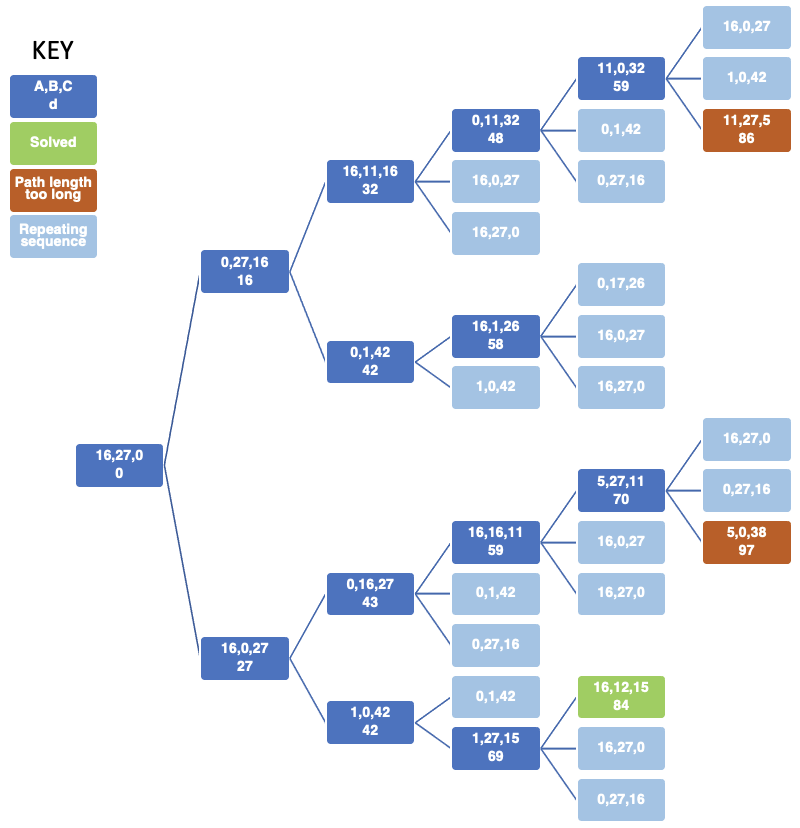
\includegraphics[]{pic1.png}
\end{proof}

\end{enumerate}
\end{required}



\newpage
\section{Standard 4- Examples Where Greedy Algorithms Fail}

\subsection{Problem \ref{GreedyFail1}}
\begin{required} \label{GreedyFail1}
Recall the \textsf{Interval Scheduling} problem, where we take as input a set of intervals $\mathcal{I}$. The goal is to find a maximum-sized set $S \subseteq \mathcal{I}$, where no two intervals in $S$ intersect. Consider the greedy algorithm where we place all of the intervals of $\mathcal{I}$ into a priority queue, ordered earliest start time to latest start time. We then construct a set $S$ by adding intervals to $S$ as we poll them from the priority queue, provided the element we polled does not intersect with any interval already in $S$. \\

\noindent Provide an example with at least $5$ intervals where this algorithm fails to yield a maximum-sized set of pairwise non-overlapping intervals. Clearly specify both the set $S$ that the algorithm constructs, as well a larger set of pairwise non-overlapping intervals. \\

\noindent You may explicitly specify the intervals by their start and end times (such as in the examples from class) or by drawing them. \textbf{If you draw them, please make it very clear whether two intervals overlap.} You are welcome to hand-draw and embed an image, provided it is legible and we do not have to rotate our screens to grade your work. Your justification should still be typed. If you would prefer to draw the intervals using \LaTeX, we have provided sample code below. \\
\end{required}


%Sample code to draw intervals
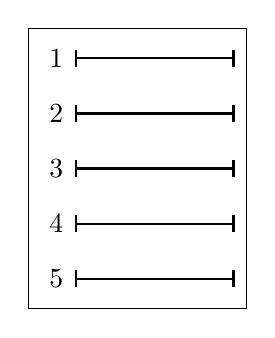
\begin{tikzpicture}[thick, framed]   
\interval{3.3}{5}{7}{1}
\interval{2.6}{5}{7}{2}
\interval{1.9}{5}{7}{3}
\interval{1.2}{5}{7}{4}
\interval{0.5}{5}{7}{5}
\end{tikzpicture}

\begin{proof}[Answer] $ $ \\ \\
\begin{tikzpicture}[thick, framed]   
\interval{3.3}{3}{10}{1}
\interval{2.6}{11}{14}{2}
\interval{1.9}{4}{5}{3}
\interval{1.2}{6}{7}{4}
\interval{0.5}{8}{13}{5}
\end{tikzpicture}
$ $ \\ \\
This is an example where the greedy algorithm will not solve the interval scheduling problem. First it will choose interval 1 because it has the earliest start time. Then it pulls interval 3,4, and 5 out of the queue but they all intersect with interval 1. Finally interval 2 is chosen because it has the next earliest start time that doesn't overlap with interval 1. However, this is incorrect because intervals 3,4, and 5 would create the maximum-sized set.
\end{proof}






\newpage
\subsection{Problem \ref{GreedyFail3}}
\begin{required} \label{GreedyFail3}
Consider now the \textsf{Weighted Interval Scheduling} problem, where each interval $i$ is specified by 
\[
([\text{start}_{i}, \text{end}_{i}], \text{weight}_{i}). 
\]

\noindent Here, the weight is an assigned value that is independent of the length $\text{end}_{i} - \text{start}_{i}$. Here, you may assume $\text{weight}_{i} > 0$. We seek a set $S$ of pairwise non-overlapping intervals that maximizes $\sum_{i \in S} \text{weight}_{i}$. That is, rather than maximizing the number of intervals, we are seeking to maximize the sum of the weights. \\

\noindent Consider a greedy algorithm which works identically as in Problem \ref{GreedyFail1}. Draw an example with at least 5 appointments where this algorithm fails. Show the order in which the algorithm selects the intervals, and also show a subset with larger weight of non-overlapping intervals than the subset output by the greedy algorithm. The same comments apply here as for Problem \ref{GreedyFail1} in terms of level of explanation.
\end{required}

\begin{proof}[Answer] $ $ \\ \\
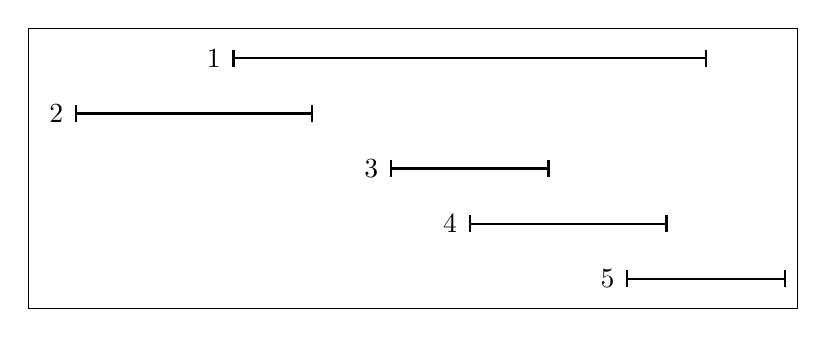
\begin{tikzpicture}[thick, framed]   
\interval{3.3}{7}{13}{1}
\interval{2.6}{5}{8}{2}
\interval{1.9}{9}{11}{3}
\interval{1.2}{10}{12.5}{4}
\interval{0.5}{12}{14}{5}
\end{tikzpicture}
\\ \\
WEIGHTS: 
\begin{enumerate}
    \item $weight_1 = 20$
    \item $weight_2 = 5$
    \item $weight_3 = 1$
    \item $weight_4 = 16$
    \item $weight_5 = 6$
\end{enumerate}

The algorithm first starts by choosing interval 2 due to its earliest start time. Continuing in ascending order of earliest start time with non-overlapping intervals, intervals 3 and 5 are chosen next. The combined weight of intervals 2,3, and 5 is 12. Therefore this example shows how the algorithm can fail because choosing interval 1 will yield a total weight of 20, which is more than 12. 
\end{proof}




\newpage
\section{Standard 5- Exchange Arguments}
\subsection{Problem \ref{Exchange1}}
\begin{required} \label{Exchange1}
Recall the Making Change problem, where we have an infinite supply of pennies (worth $1$ cent), nickels (worth $5$ cents), dimes (worth $10$ cents), and quarters (worth $25$ cents). We take as input an integer $n \geq 0$. The goal is to make change for $n$ using the fewest number of coins possible. \\

\noindent Prove that in an optimal solution, we use at most $2$ dimes. 
\end{required}

\begin{proof}
\begin{lstlisting}
Exchange argument

    Proposed optimal solution
    # of pennies = p (p $\leq$ 4) 
    # of nickels = n (n $\leq$ 1)
    # of dimes = d (d $\leq$ 2) 
    # of quarters = q
    total # of coins = p+n+d+q
    
    Say in our optimal example that d=2. For our exchange argument, we want to
    have the same amount of money but d=3. 

    Proposed optimal example
    # of pennies = p
    # of nickels = n
    # of dimes = 2
    # of quarters = q
    total # of coins = p+n+q+2
    
    Exchange example
    # of pennies = p
    # of nickels = n+3  
    # of dimes = 3
    # of quarters = q-1
    total # of coins = p+n+3+3+q-1 = p+n+q+5
    
    The only way to exchange 2 dimes with 3 dimes is to take away a quarter
    first. Then from these 25 cents, adding a dime leaves us with 15 cents.
    Only using nickels and pennies, the smallest number of coins you can now
    add is 3 nickels. 
    
    From the total number of coins, p+n+q+5 > p+n+q+2. Therefore, the optimal
    solution uses at most 2 dimes because using more than 2 dimes will 
    increase the total amount of coins. 
    
    This will also hold true for d>3 because in order to add dimes, you
    always need to remove quarters. This then will add more pennies and/or 
    nickels than quarters being removed, resulting in more overall coins. 
    
\end{lstlisting}




\end{proof}



\newpage
\subsection{Problem \ref{Exchange2}}

\begin{required} \label{Exchange2}
Consider the \textsf{Interval Projection} problem, which is defined as follows.
\begin{itemize}
\item \textsf{Instance:} Let $\mathcal{I}$ be a set of intervals on the real line.
\item \textsf{Solution:} A minimum sized set $S$ of points on the real line, such that (i) for every interval $[s, f] \in \mathcal{I}$, there exists a point $x \in S$ where $x$ is in the interval $[s, f]$. We call $S$ a \textit{projection set}.
\end{itemize}

\noindent Do the following.
\begin{enumerate}[label=(\alph*)]
\subsubsection{Problem 7\ref{6a}}
\item \label{6a} Find a minimum sized projection set $S$ for the following set of intervals:
\begin{align*}
\mathcal{I} = \{ [0, 1], [0.5, 1], [1, 1.5], [1.4, 2], [1.6, 2.3] \}.
\end{align*}


\begin{proof}[Answer]
$S = \{1,1.8\}$
\end{proof}

\newpage
\subsubsection{Problem 7\ref{6b}}
\item \label{6b} Fix a set of intervals $\mathcal{I}$, and let $S$ be a projection set. Prove that there exists a projection set $S^{\prime}$ such that (i) $|S^{\prime}| = |S|$, and (ii) where every point $x \in S^{\prime}$ is the right end-point of some interval $[s, f] \in \mathcal{I}$. 

\begin{proof} $ $ \\ 

\begin{enumerate}
    \item Using the interval scheduling algorithm: let the set $M \subseteq I$ be the maximum sized set of intervals. Assume that if an interval ends at the exact time another interval starts then they are considered as overlapping. 
    \item The cardinality of the set $M$ is equivalent to the number of points in $S$.
    \item This is because $|M|$ represents the maximum number of sets that do not overlap. Therefore, there must be a point within each of the intervals in M to solve the interval projection problem. 
    \item The rest of the intervals will contain at least one of the points because they overlap with at least one the intervals in $M$.
    \item Using this fact, the points that lie on the intervals in $M$ can be anywhere on those intervals, including the end point of the interval.
    \item Therefore, if all the points of $S'$ are on the end points, then $|S|$ is still equal to $|S'|$ because they are both equal to $|M|$ 
\end{enumerate}

For example: \\ \\
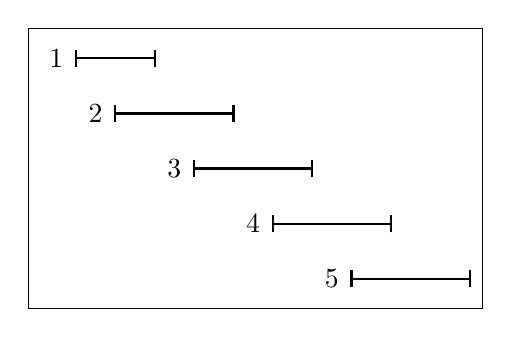
\begin{tikzpicture}[thick, framed]   
\interval{3.3}{7}{8}{1}
\interval{2.6}{7.5}{9}{2}
\interval{1.9}{8.5}{10}{3}
\interval{1.2}{9.5}{11}{4}
\interval{0.5}{10.5}{12}{5}
\end{tikzpicture} \\ \\
$M = \{1,3,5\}$ and $|M| = 3$ \\
As explained above, there must be a point that lies in 1, 3, and 5. Whether or not these points are on the end point of the interval or not, they can still work. So, $|S| = 3$ and $|S'| = 3$

\end{proof}

\end{enumerate}
\end{required}
 
\end{document} % NOTHING AFTER THIS LINE IS PART OF THE DOCUMENT



